\documentclass{standalone}
\usepackage{tikz}
\usepackage{multirow}
\usepackage{multicol}
\usepackage[margin=1in]{geometry}

\usetikzlibrary{fit}

\begin{document}
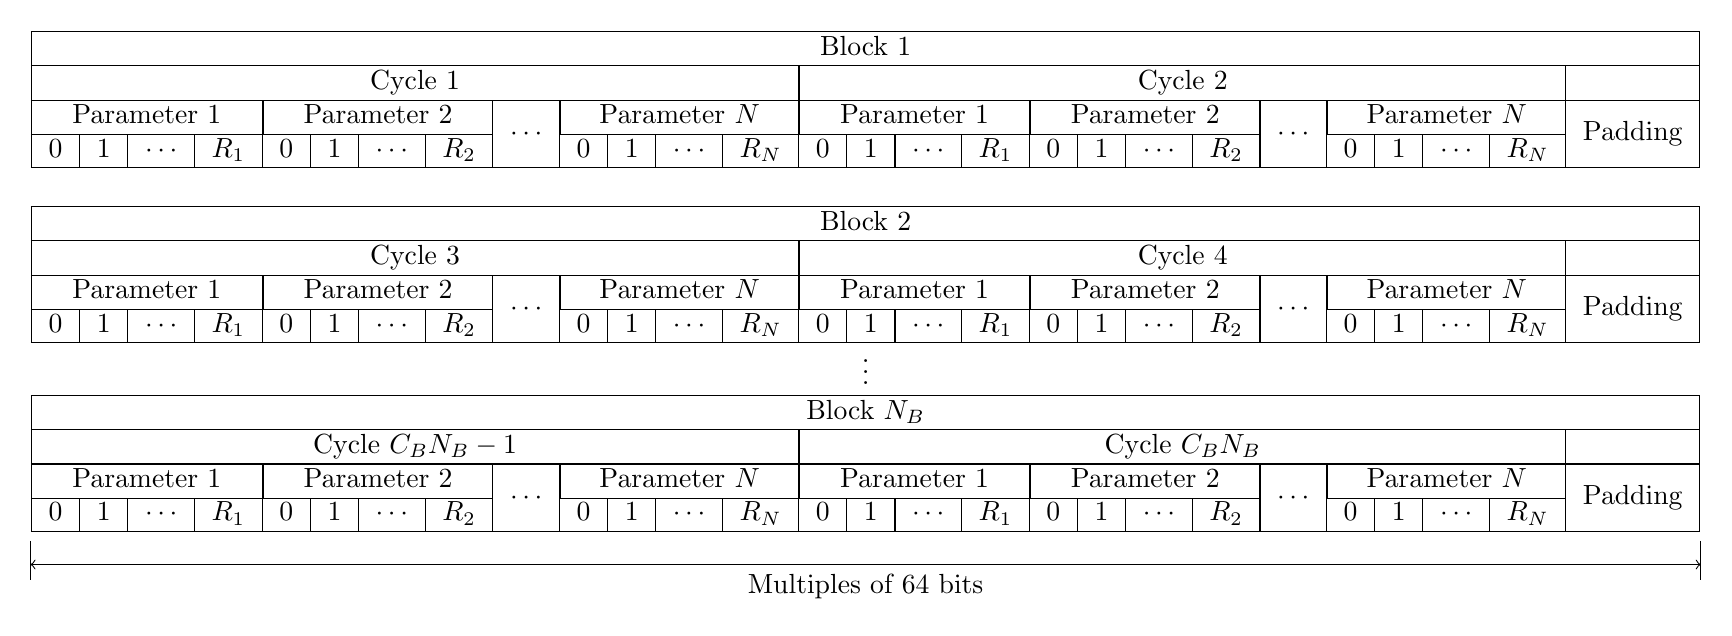
\begin{tikzpicture}
\node (table) [inner sep=0pt] {
	\begin{tabular}{@{}|c|c|c|c|c|c|c|c|c|c|c|c|c|c|c|c|c|c|c|c|c|c|c|c|c|c|c|@{}}
		\hline
			\multicolumn{27}{|c|}{Block \(1\)} \\
		\hline
			\multicolumn{13}{|c|}{Cycle \(1\)} &
			\multicolumn{13}{|c|}{Cycle \(2\)} & \\
		\hline
		% Cycle 1
			\multicolumn{4}{|c|}{Parameter \(1\)} &
			\multicolumn{4}{|c|}{Parameter \(2\)} &
			\multirow{2}{*}{\(\cdots\)} &
			\multicolumn{4}{|c|}{Parameter \(N\)} &
		% Cycle 2
			\multicolumn{4}{|c|}{Parameter \(1\)} &
			\multicolumn{4}{|c|}{Parameter \(2\)} &
			\multirow{2}{*}{\(\cdots\)} &
			\multicolumn{4}{|c|}{Parameter \(N\)} &
			\multirow{2}{*}{Padding} \\
		\cline{1-8}
		\cline{10-21}
		\cline{23-26}
		% Cycle 1
			0 & 1 & \(\cdots\) & \(R_1\) &
			0 & 1 & \(\cdots\) & \(R_2\) & &
			0 & 1 & \(\cdots\) & \(R_N\) &
		% Cycle 2
			0 & 1 & \(\cdots\) & \(R_1\) &
			0 & 1 & \(\cdots\) & \(R_2\) & &
			0 & 1 & \(\cdots\) & \(R_N\) & \\
		\hline
		\multicolumn{8}{c}{\raisebox{1em}{}} \\
		\hline
			\multicolumn{27}{|c|}{Block \(2\)} \\
		\hline
			\multicolumn{13}{|c|}{Cycle \(3\)} &
			\multicolumn{13}{|c|}{Cycle \(4\)} & \\
		\hline
		% Cycle 1
			\multicolumn{4}{|c|}{Parameter \(1\)} &
			\multicolumn{4}{|c|}{Parameter \(2\)} &
			\multirow{2}{*}{\(\cdots\)} &
			\multicolumn{4}{|c|}{Parameter \(N\)} &
		% Cycle 2
			\multicolumn{4}{|c|}{Parameter \(1\)} &
			\multicolumn{4}{|c|}{Parameter \(2\)} &
			\multirow{2}{*}{\(\cdots\)} &
			\multicolumn{4}{|c|}{Parameter \(N\)} &
			\multirow{2}{*}{Padding} \\
		\cline{1-8}
		\cline{10-21}
		\cline{23-26}
		% Cycle 1
			0 & 1 & \(\cdots\) & \(R_1\) &
			0 & 1 & \(\cdots\) & \(R_2\) & &
			0 & 1 & \(\cdots\) & \(R_N\) &
		% Cycle 2
			0 & 1 & \(\cdots\) & \(R_1\) &
			0 & 1 & \(\cdots\) & \(R_2\) & &
			0 & 1 & \(\cdots\) & \(R_N\) & \\
		\hline
		\multicolumn{27}{c}{\(\vdots\)} \\
		\hline
			\multicolumn{27}{|c|}{Block \(N_B\)} \\
		\hline
			\multicolumn{13}{|c|}{Cycle \(C_B N_B - 1\)} &
			\multicolumn{13}{|c|}{Cycle \(C_B N_B\)} & \\
		\hline
		% Cycle 1
			\multicolumn{4}{|c|}{Parameter \(1\)} &
			\multicolumn{4}{|c|}{Parameter \(2\)} &
			\multirow{2}{*}{\(\cdots\)} &
			\multicolumn{4}{|c|}{Parameter \(N\)} &
		% Cycle 2
			\multicolumn{4}{|c|}{Parameter \(1\)} &
			\multicolumn{4}{|c|}{Parameter \(2\)} &
			\multirow{2}{*}{\(\cdots\)} &
			\multicolumn{4}{|c|}{Parameter \(N\)} &
			\multirow{2}{*}{Padding} \\
		\cline{1-8}
		\cline{10-21}
		\cline{23-26}
		% Cycle 1
			0 & 1 & \(\cdots\) & \(R_1\) &
			0 & 1 & \(\cdots\) & \(R_2\) & &
			0 & 1 & \(\cdots\) & \(R_N\) &
		% Cycle 2
			0 & 1 & \(\cdots\) & \(R_1\) &
			0 & 1 & \(\cdots\) & \(R_2\) & &
			0 & 1 & \(\cdots\) & \(R_N\) & \\
		\hline
	\end{tabular}};
	\foreach \i/\corner in {1/south west, 2/south east}
		\draw (table.\corner) ++(down:3pt) -- ++(down:0.3cm)
		      coordinate (p\i) -- ++(down:0.2cm);
	\draw [<->] (p1) -- (p2)
	      node [midway,anchor=north] {Multiples of 64 bits};
	% The right dimension line gets cut off otherwise.
	\node [fit=(table),inner sep=1pt] {};
\end{tikzpicture}
\end{document}
